\graphicspath{{chapters/07/images/}}
\chapter{Reali}

\hypertarget{introduction}{%
\section{Introduction}\label{introduction}}

The course follows the structure of the article
\textbf{\emph{Optimization Algorithms for Computational Systems
Biology.}}

\hypertarget{definition-of-a-system}{%
\subsection{Definition of a system}\label{definition-of-a-system}}

A system is a set of integrated and interacting \emph{components} or
\emph{entities} that form a whole with definite boundaries and
surrounding environment. A system has a goal to achieve by performing
one or more functions or tasks. Systems can be aggregated into a
\textbf{\emph{hierarchy}}. A system at a given level of detail can be a
component at a higher level of detail.

\begin{itemize}
\tightlist
\item
  A \textbf{\emph{complex}} (non-linear) \textbf{\emph{system}} is a
  system that does not satisfy the principle of superposition, i.e., the
  behavior of the system cannot be inferred from the behavior of its
  components.
\item
  A \textbf{\emph{dynamical system}} is a system where fixed rules
  define the time dependencies of the system in a geometrical space.
  Dynamical systems have a space and time dimension because they change
  their characteristics over time. If we pick snapshots of the system at
  different time points, we observe different configurations of the
  system (data).
\end{itemize}

A \textbf{\emph{configuration}} or state of the system refers to the
current condition of the system and stores enough information to predict
its next move. A state is characterized by the position of its
components in a geometrical space and by the values of the attributes of
its components (e.g., concentration or number of each elements
involved). Systems change their state over time by changing the location
of some of their components or changing the attributes of some of their
components.

\begin{itemize}
\tightlist
\item
  \textbf{\emph{steady state}}: some of the attributes of the system are
  no longer changing in the future.
\item
  transient state: time needed to reach the steady state.
\end{itemize}

\hypertarget{determinism-nondeterminism-or-stochasticity}{%
\subsection{Determinism, nondeterminism, or
stochasticity?}\label{determinism-nondeterminism-or-stochasticity}}

\begin{itemize}
\tightlist
\item
  \textbf{\emph{Deterministic systems}} always react in the same way to
  the same set of stimuli. These systems are completely determined by
  the initial state and the input set. The essence of deterministic
  systems is that each event is causally related to previous events and
  choices are always resolved in the same way in the same context. When
  a system generates multiple outcomes from the same input in different
  observations, the system is \textbf{\emph{nondeterministic}} (we
  cannot predict the output from the input).
\item
  \textbf{\emph{Stochasticity}} is the quality of lacking any
  predictable order or plan and stochastic systems possess some inherent
  randomness. It is possible to transform a nondeterministic system into
  a stochastic one by attaching probabilities to the selection points so
  that we turn nondeterministic choices into probabilistic choices.
\end{itemize}

\hypertarget{computational-complexity}{%
\subsection{Computational
complexity}\label{computational-complexity}}

Complexity arises when interacting components self-organize to form
evolving structures that exhibit a hierarchy of emergent system
properties. An \textbf{\emph{emergent behavior}} can be originated by a
collection of components that interact in the absence of a centralized
point of control to produce something that has not been designed or
programmed in the system construction or evolution. Example: internet,
ant colonies, consciousness.\\
\textbf{\emph{Computational complexity}} is the amount of resources,
measured as a function of the size of the input, needed to execute an
algorithm.

\begin{itemize}
\tightlist
\item
  Computational space complexity: the amount of memory needed;
\item
  Computational time complexity: the number of instructions to be
  executed.
\end{itemize}

\hypertarget{definition-of-a-model}{%
\subsection{Definition of a model}\label{definition-of-a-model}}

A \emph{representation} is a set of symbols used to convey information
and knowledge about a system. It is either physical as a cell or an
ecosystem, or artificial as a computer network or an economic market. An
abstraction is a representation that ignores some aspects of a system
which are not of interest for the current investigation.

A model is an abstraction of a system. A model has its own interacting
components that are characterized by the attributes that we want to
observe. The set of all the attributes in a model is the
\emph{experimental frame}.

\begin{itemize}
\item
  A \emph{dynamic model} aims at predicting the behavior of the system
  in time/space through what if analysis. What if analysis investigates
  how a change in some attributes affects the behavior of the modeled
  system.
\item
  A \emph{computational model} is a model that can be manipulated by a
  computer to observe properties of the corresponding system.

  \begin{figure}
  \centering
  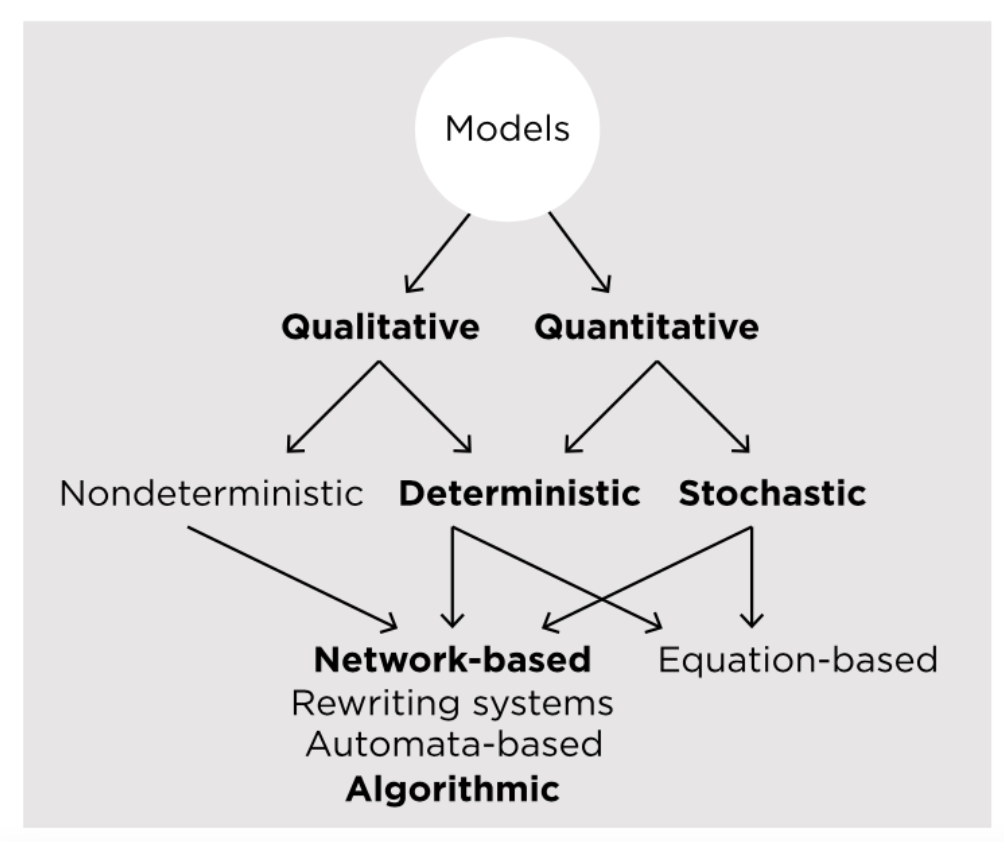
\includegraphics{scheme_model.png}
  \caption{scheme\_model}
  \end{figure}
\end{itemize}

\hypertarget{checking-the-validity-of-a-model}{%
\subsection{Checking the validity of a
model}\label{checking-the-validity-of-a-model}}

\emph{Validity} is a fundamental property of models and witnesses the
capacity of a model of making good predictions because the model soundly
captures the aspects of interest. We need to assess the validity of a
model before using it to predict the behavior of a system.

Assume that $M$ is a model for the system $S$ and $\underline{M}$ is the
modeling process. Let $s(t)$ and $m(t)$ be the state of the system and
of the model at time $t$, and $f_s$ and $f_m$ the state transition
functions of the system and of the model, respectively. Finally, let
$I_s(t)$ and $O_s(t)$ be the input and output of the system at time $t$.
Similarly, we write $I_m(t)$ and $O_m(t)$ for the model.

What we expect is that going from one state to the other we have a
function (one for the system and one for the model); in a mathematical
model we integrate the $f_m$ function to known what happens in the
transition of the model, but we cannot do that in the real setting (the
transition function $f_s$ is not known) → when dealing with nature, we
cannot validate models according to the previous definition, so we use
I/O validity, based on known input and outputs of the system.

The input and output are here generalized concepts: input can be any
perturbation of the system or of the model and output can be any
observable property causally related to the input.

A model $M$ is valid for a system $S$ if:
$f_m(\underline{M}(s(t_0))) = \underline{M}(f_s(s(t_0))) = m(t_1)$

\begin{figure}
\centering
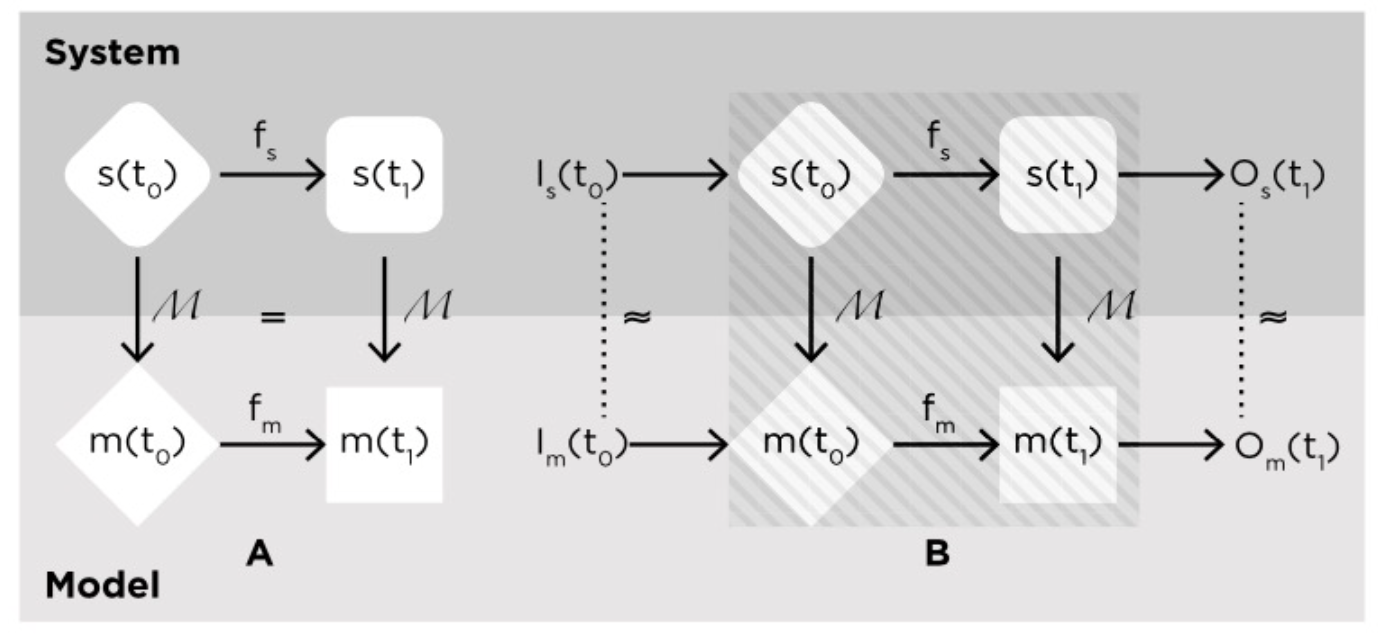
\includegraphics{validation.png}
\caption{validiation}
\end{figure}

I/O validity can be checked by using data sets produced by the model and
observed and measured on the system. An issue in this comparison process
is \emph{overfitting}:

\begin{itemize}
\tightlist
\item
  a model is well tuned to a specific dataset used to build the model
\item
  it performs poorly on other datasets
\end{itemize}

\textbf{Cross-validation}: check overfitting by testing the model on
data sets different from the ones used to build and calibrate/train the
model.

These concepts, even if usually referred to computational models, may
apply to general models or representations of a system.

\hypertarget{how-to-build-a-model}{%
\subsection{How to build a model}\label{how-to-build-a-model}}

We need to define objectives:

\begin{itemize}
\tightlist
\item
  what do you want to model?
\item
  what do you want to investigate with the model?
\item
  what do you expect from the model?
\item
  why do you need a model?
\end{itemize}

\begin{figure}
\centering
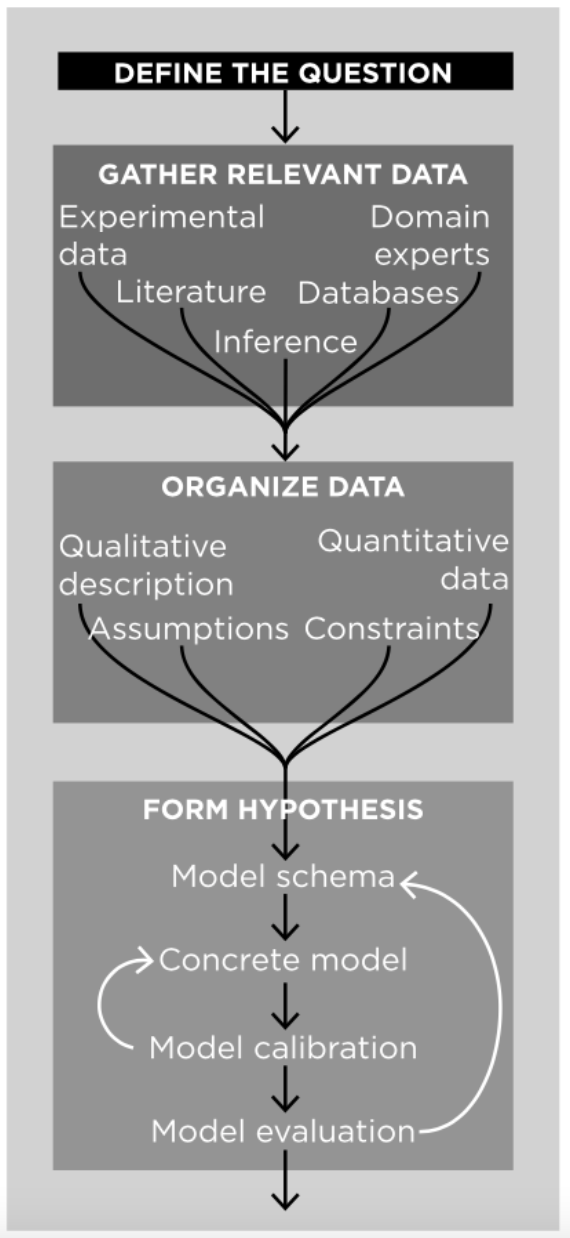
\includegraphics{workflow.png}
\caption{workflow}
\end{figure}

After defining the question and gathering data, we need to build the
model and calibrate it, in order to check if it can recapitulate data.
If it does not, either we are missing something or we must tune some
parameters. Different parameters can lead to dramatic changes in
dynamics. Example: Lotka-Volterra model with different parameter
conditions:

\begin{figure}
\centering
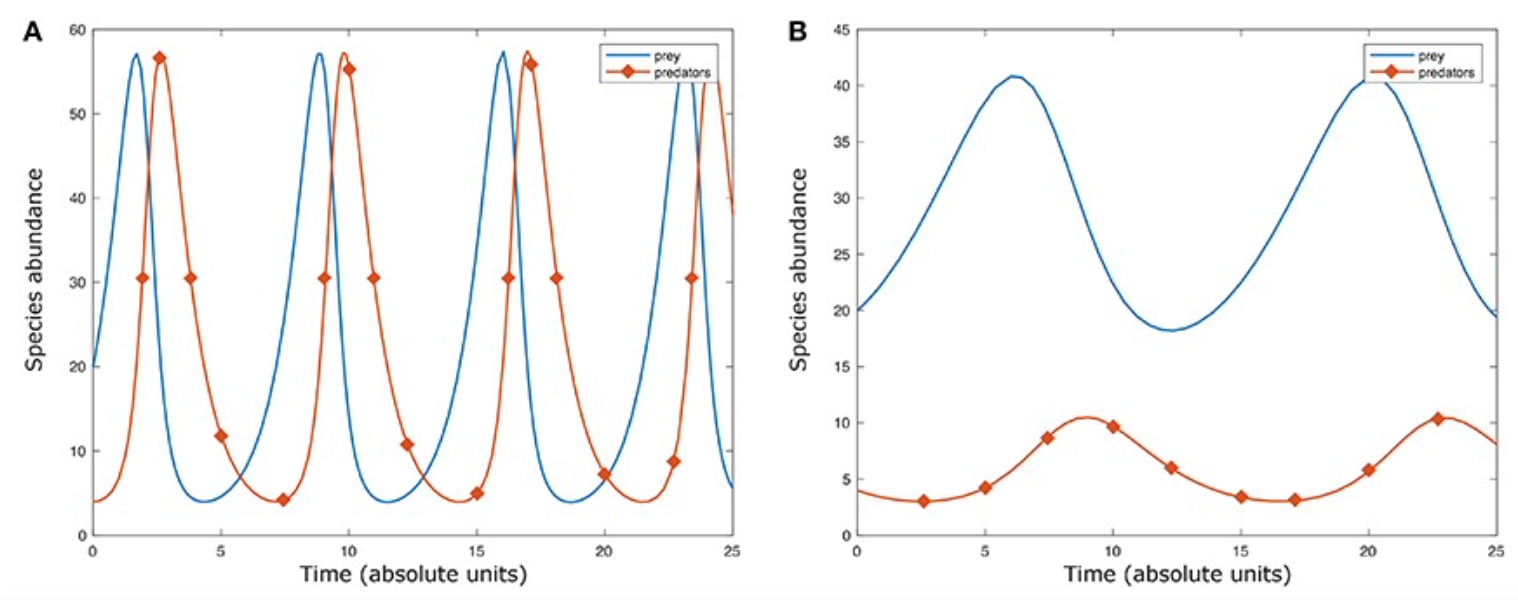
\includegraphics{volterra.png}
\caption{volterra}
\end{figure}

\begin{enumerate}
\def\labelenumi{\Alph{enumi})}
\item
  shows periodic oscillations, same amount of preys and predators
\item
  wider peaks and lower predator presence
\end{enumerate}

\hypertarget{optimization-problem}{%
\section{Optimization problem}\label{optimization-problem}}

In general, it is a problem in which we try to maximize or minimize
something. What we want to optimize is a function usually called
objective function (or cost function). The function depends on a
variable or a vector of variables), called unknowns or parameters or
parameter estimates. They may be subject to certain
constraints(\textless,\textgreater,=).

\hypertarget{general-definition-of-an-optimization-problem}{%
\subsection{General definition of an optimization
problem}\label{general-definition-of-an-optimization-problem}}

$\left.\left\{\begin{array}{ll} \max _{x \in \mathbb{R}^n} f(x) & \\ c_i(x)=0 & i=\mathcal{E}\\ f_j(x) \geq 0 & j = I \end{array}\right\} \text { set of indexes }\right] \text { Constraints (equality and inequality) }$

The model (for us) is a function that gives a certain interval/time,
initial conditions and parameters, returns the variables at that time.
(Assume deterministic description)

$m: \mathbb{R} \times \mathbb{R}^{(n+1)} \times \mathbb{R}^m \rightarrow \mathbb{R}^N$

where n+1 accounts for the dimension of variables and time.

$$
\left(t_1,\left(\vec{x}_0, t_0\right), \theta\right)
\longmapsto \vec{x}_1 $$

Initial conditions in Lotka-Volterra: $((20,5), 0)$. $\theta$ represents
parameters e.g.~in Lotka-Volterra, $a,b,\beta,\alpha$.

Now, assume that we have $k$ observations:

$(t_i ,\vec{y}_i), i=1, \ldots k$ , where
$t_i \in \mathbb{R}^+, \vec{y}_i \in \mathbb{R}^\ell$

$y$ in theory can be a subset, $\ell<N$ : this happens a lot in complex
systems, we may not observe all variables! For simplicity, we can assume
$\ell=N$. Assuming that we can compute the following:

$*m\left(t_1,\left(\vec{x}_0, t_0\right), \theta\right) \in \mathbb{R}^{N} =_{\text{drop initial point notation}} m(t_i,\theta)*$

We can compute distance: \emph{$d_i=\vec{y}_i-m(t_i, \theta)$}

We can choose any type of distance (Euclidean, max\ldots). What we do is
calculate point-wise the distance between the model and `true' labels.
It is quite common to use the \textbf{\emph{Euclidean distance}}:
$*d \varepsilon =\sqrt{\sum_{i=1}^k(\vec{y}_i,-m(t_i, \theta))^2}$
$\rightarrow d{\varepsilon}-\sqrt{\sum_{i=1}^{K} \sum_{j=1}^{N} \left(y_{ij}-m_j\left(t_i, \theta\right)\right)^2}$*
Sometimes we need need to add weights, which multiply each component in
the distances. We are putting together many outputs from the same model,
so we might want to scale everything to make it more comparable.
Furthermore, variables might be in different units of measurement,
leading to biased results.

Observations:

\begin{itemize}
\tightlist
\item
  we do not want to reach ``zero'' when minimizing. Indeed, if the
  residual error $=0$, we are $100 \%$ sure that we are overfitting the
  data.
\item
  we need to really understand the data to construct the model
\item
  we are manipulating $\theta$ in the space of the parameters, but we
  modify the output in the space of the observations: we are connecting
  abstract values to observations - like parameters for maximum
  likelihood.
\end{itemize}

Weights are multiplicative factors, sometimes we might wish to
\emph{transform} the distance.

\textbf{Least squares algorithm}

$d{\varepsilon}=\sqrt{\sum \sum W_{ij}\left(y_{ij}-m_j\left(t_i, \theta\right)\right)}$

LECTURE 2

Our problem is to minimize/maximize a function.

Assume

$$
\min f(x), x \in \mathbb{R}^n
$$

\hypertarget{definition-of-a-minimum}{%
\subsection{Definition of a minimum}\label{definition-of-a-minimum}}

A point $x^*$ is called \textbf{minimum} if
$\exists \varepsilon > 0 : \forall x : || x- x^* || < \varepsilon$

$$
\Rightarrow f(x) \geq f(x^*) \\ 
$$

{[}For the maximum $f(x) \leq f(x^*)${]}

The minimum is \textbf{\emph{global}} if $\forall x \in \mathbb{R}^n$
(or in our domain) $f(x) \geq f(x^*)$. In general it is not easy to
determine global minimum/maximum, especially if we have a lot of
dimensions.

To find minima or maxima, we should impose $f'(x)=0$.

We call a \textbf{\emph{stationary point}}, a
$\bar{x} \text{ s.t.} f'(\bar{x})=0$.

\hypertarget{gradient-methods}{%
\section{Gradient methods}\label{gradient-methods}}

When we integrate to find ODE solutions, we do not obtain a function as
a solution, just points.

In our optimization problem we do not know $f$ and $f'$(only sometimes
we do), so we are required to use numerical approximation. The idea of
looking at $f'$ and set $f'=0$ is still at the base of gradient methods.

If the problem contains constraints, how do we solve it? In this case
the problem is:

$$\left\{\begin{array}{ll}
\max f(x) &  \\
g_i(x)=0, & i \in \mathcal{I} \\
x \in \mathbb{R}^N
\end{array}\right.$$

Let $\mathcal{I}= 1,...,m$. The traditional way to solve this problem is
to translate this system to another function. The Lagrangian function is
used to take into account the constraints.

\hypertarget{lagrangian-function}{%
\subsubsection{Lagrangian function}\label{lagrangian-function}}

We define the \textbf{\emph{Lagrangian function}} as
$L: \mathbb{R}^n \times \mathbb{R}^m \rightarrow \mathbb{R}$ s.t.

$$
L(x)= f(x) + \lambda g(x) = f(x) + \sum_{j=1}^m \lambda_j g_j(x)
$$

\hypertarget{lagrangian-multipliers-theorem}{%
\subsection{Lagrangian Multipliers
Theorem}\label{lagrangian-multipliers-theorem}}

If $x^*$ is a stationary point for (Lagrangian function), then
$\exists \lambda^*$ s.t. $(x^* \lambda^*)$ is a stationary point for L. It
is a necessary condition (not sufficient, only one direction).

This is a ``bigger'' problem, from
$\mathbb{R}^N \rightarrow \mathbb{R}^N \times \mathbb{R}^m$ . But still,
I can search solutions using stationary points. We can generalize the
idea to $g_i(x) \leq 0,$ constraints

Remember that stationary points are not necessarily minima and maxima.
We check whether a stationary point is a max/min through second
derivations or evaluate the function in ``other'' points.

\hypertarget{definition-of-a-gradient}{%
\subsection{Definition of a
gradient}\label{definition-of-a-gradient}}

Let $f: \mathbb{R}^N \rightarrow \mathbb{R}$ a differentiable function,
we call gradient of $f$

$\nabla f: \mathbb{R}^N \rightarrow \mathbb{R}^N$ sit.
$\nabla f_i=\frac{\partial}{\partial x_i} f(x)_i$ and
$\nabla f(x) =\left[\begin{array}{c}\frac{\partial}{\partial x_1} f(x) \\ \vdots \\ \frac{y}{\partial x_N} f(x)\end{array}\right]$
We look for points for which the derivative vanishes
$x^* : \nabla f(x^*)=0$

TRY at
home:$f(x, y)=(1-x)^2+100\left(y-x^2\right)^2 \\ f(x, y)=-(y+47) \sin \left(\sqrt{\left.\mid \frac{x}{2}+(y+47)\right|}-\right. x \cdot \sin \left(\sqrt{\left.\mid x-(y+47\right)|}\right).$

These two functions are used to test optimization algorithms. The first
is \textbf{Rosenbrock's function,} the second the \textbf{Eggholder
function}. Solving analytically these problems is hard.

We cannot apply gradient methods for stochastic simulations, since the
function is not continuous.

\hypertarget{limitations-of-gradient-descent-methods}{%
\subsection{Limitations of gradient descent
methods}\label{limitations-of-gradient-descent-methods}}

One of the major limitations of these algorithms is that we are focusing
on local minima, we never know if the distance is minimum. Furthermore,
sometimes we want to optimize more variables and it might not be optimal
to perfectly fit the solution to both of them → trade-off.

\hypertarget{discussion}{%
\subsection{Discussion}\label{discussion}}

If we have an equality constraint we are only considering the points
meeting the boundary (red). In an inequality constraint, we consider
everything inside the red circle (yellow area). Generally, constraints
reduce our search space; the Lagrangian tells us that the minimum point
with some multipliers will give a solution of the Lagrangian, which is
one function. If we find the solutions, we do not know if they are
solutions of the original conditions, but they are ideal candidates that
can then be checked.

\begin{figure}
\centering
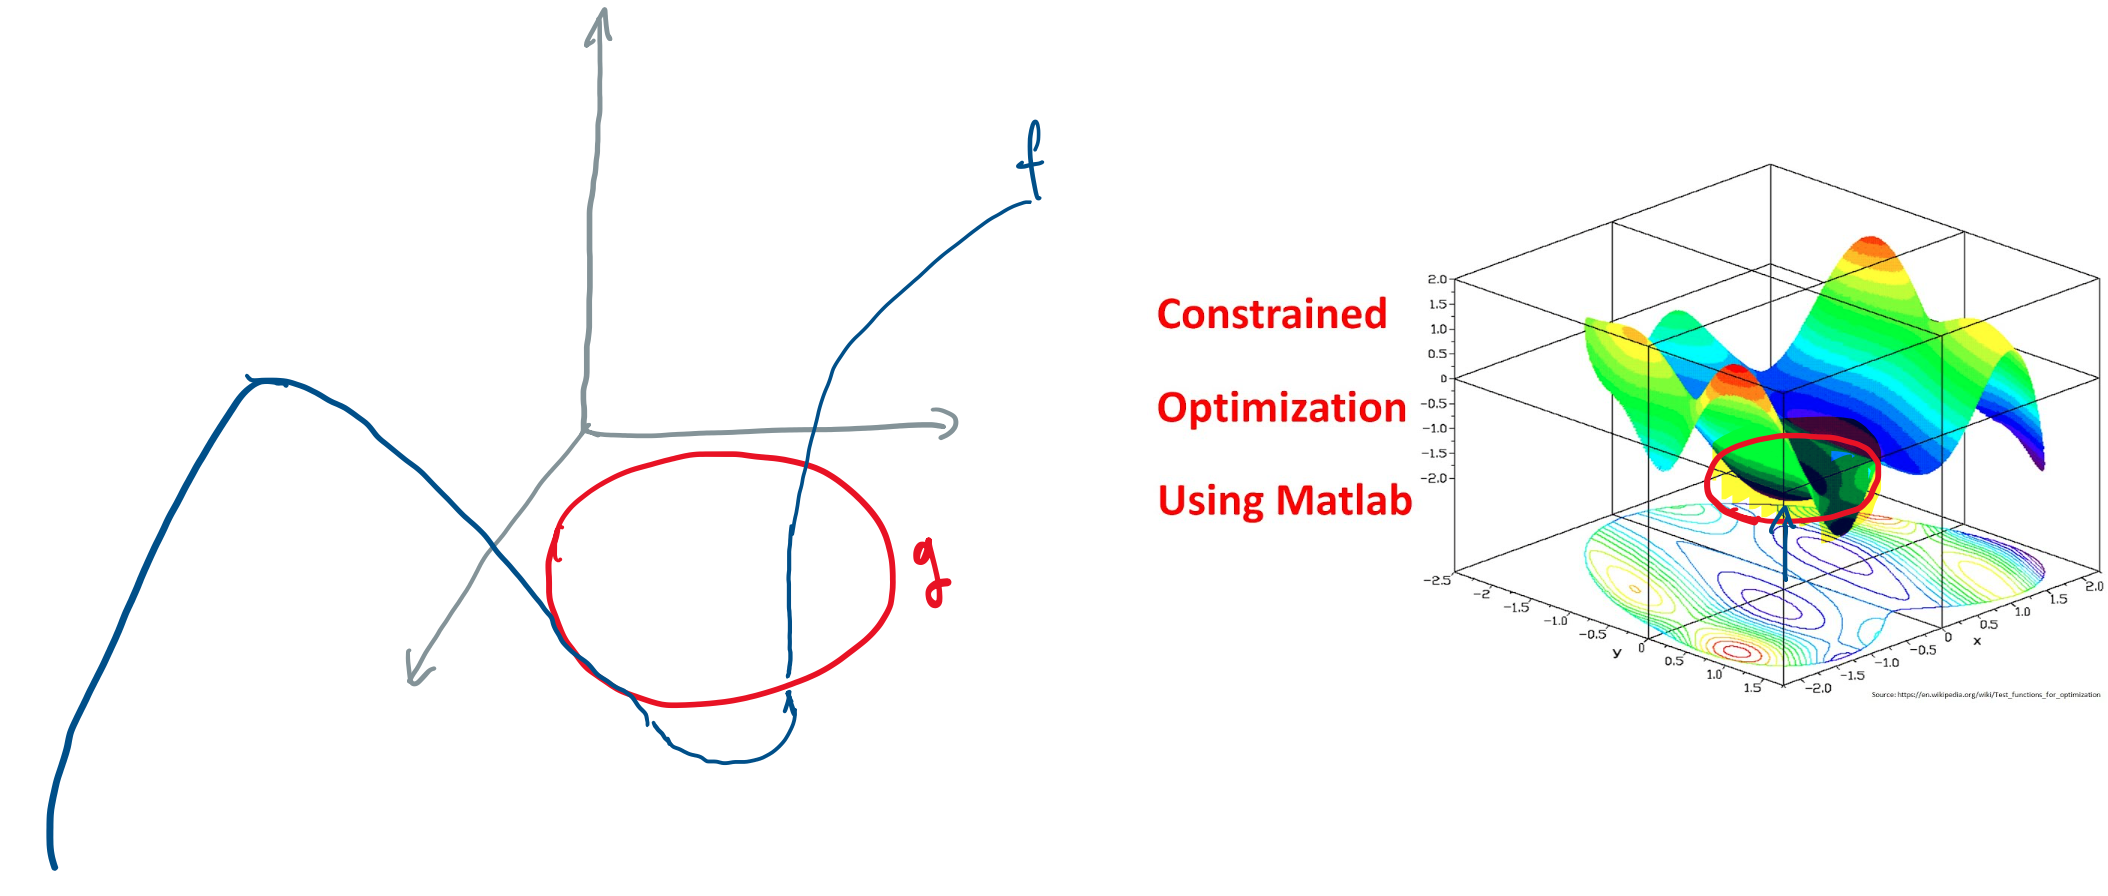
\includegraphics{example.png}
\caption{Blue = function, red = constraint}
\end{figure}

Blue = function, red = constraint

For performing an evaluation of the distance we should integrate the
model, which is computationally expensive. To do one integration we must
perform a lot of computations. Our measure of computational cost is the
number of times we have to simulate the model (per iteration).

In most cases, we do not know the gradient, therefore we should
approximate it using the Taylor formula.

\hypertarget{gradient-approximation-with-taylor-formula}{%
\subsection{Gradient approximation with Taylor
formula}\label{gradient-approximation-with-taylor-formula}}

$(a,b) \in \mathbb{R}, x_0 \in (a,b)$

Let $f_i(a,b) \rightarrow \mathbb{R}$ be differentiable $(n-1)$ times in
$(a,b)$ and $f^{(n)}$ is continuous in $x_0$. Then let $x \in (a,b)$ ,
we have:

$$
f(x)=f\left(x_0\right)+f^{\prime}\left(x_0\right)\left(x-x_0\right)+f''(x_0)\frac{(x-x_0)^2}{2!}+ ...+ f^{(n)}(x_0)\frac{(x-x_0)^n}{n!} + R_n(x) \text{ s.t.} \lim_{x \rightarrow x_0} \frac{R_n(x)}{(x-x_0)^n} =0 
$$

We focus on the first terms
$f(x)=f\left(x_0\right)+f^{\prime}\left(x_0\right)\left(x-x_0\right)+R_2(x)=0 \\ f^{\prime}\left(x_0\right)=\frac{f(x)-f\left(x_0\right)}{x-x_0}+\left(\frac{R_2(x)}{\left(x-x_0\right)}-R_1(x)\right.$

! sistemare, R\_1(x) può approssimare il ratio di R\_2(x)

We can also use this trick for $N>1$

Let $f: \mathbb{R}^N \rightarrow \mathbb{R}$ and
$e_i=(0, \ldots, 0,1,0,\ldots,0)$

Let's consider $x_1 x+\varepsilon e_i, x-\varepsilon e_i$ ; we are only
moving along one direction.

In this
case:$f\left(x+\varepsilon e_i\right)=f(x)+\varepsilon \frac{\partial f}{\partial x_i}(x)+\frac{1}{2} \varepsilon^2 \frac{\partial^2 f}{\partial x_i{ }^2}(x)+R_3(x) \\ f\left(x-\varepsilon e_i\right)=f(x)-\varepsilon \frac{\partial f}{\partial x_i}(x)+\frac{1}{2} \varepsilon^2 \frac{\partial^2 f}{\partial x_i{ }^2}(x)+R_3(x) \\ \Rightarrow f\left(x+\varepsilon e_i\right)-f\left(x-\varepsilon e_i\right)=+2 \varepsilon \frac{\partial f}{\partial x_i}(x)+R_3(x) \\ \Rightarrow \frac{\partial f}{\partial x_i}(x)=\frac{f\left(x+\varepsilon e_i\right)-f\left(x-\varepsilon e_i\right)}{2 \varepsilon}+R_2(x)$

We have computed an approximation of the first derivative with improved
accuracy.

Consider that this only applies to one derivative, we have to perform
this at least twice → 2 function evaluation for each $i \Rightarrow 2W$.
In order to obtain a decent gradient, we require a lot of computations,
but they are fast (quite low number of iterations). We will see other
methods, which are somehow more precise, but also heavier.

We can always check $\Delta f=0$ or not to understand if we are done!

As we already saw, there might be points where the gradient vanishes
which are not the final destination. Gradient methods may tend to
overfitting, but they are effective. The main issue is that since we
approximate the gradient, we do not trust it everywhere.
